\subsection{The Freemium Business Model}
The group has agreed upon using a Freemium business model, where the product is given away for free for non-commercial uses. \cite{kumar, torres}.\\

The Freemium business model also help users and businesses into the platform, which is vital for this product to properly work, since some of the contents on the platform will be user submitted (Crowd Sourced).\\

To persuade more users to join, there will be an incentive programme, which allows users to invite their friends to the platform, in exchange for offers from the businesses.\\


There have also been some discussion about a premium subscription for businesses, which provides a set of premium features, targeted at the businesses who can use the platform to increase their own value.
The business premium subscription would contain features, which promotes the business subscribers through the platform, and makes them more visible for the users.
To persuade businesses to subscribe, there could be a trial period, where they can use the business features of the system for free, and afterwards decide whether they will continue their subscription, or not.
During the trial the businesses could make their existing customers aware of the platform, and get more users onto the platform that way.\\


To summarize, the application will be free to use. 
Free users can invite friends to the platform, for an exchange of good offers.
Businesses can sign up for a monthly subscription for a Business premium membership, which makes them more visible for users on the platform.

\subsection{Osterwalder Business Canvas}
The Osterwalder Business Canvas (shown in \autoref{fig:bcanvas}) can be used to analyze a business, to see where its core values lie, and where they earn their money \cite{bcanvas}.


\begin{figure}[H]
  \centering
  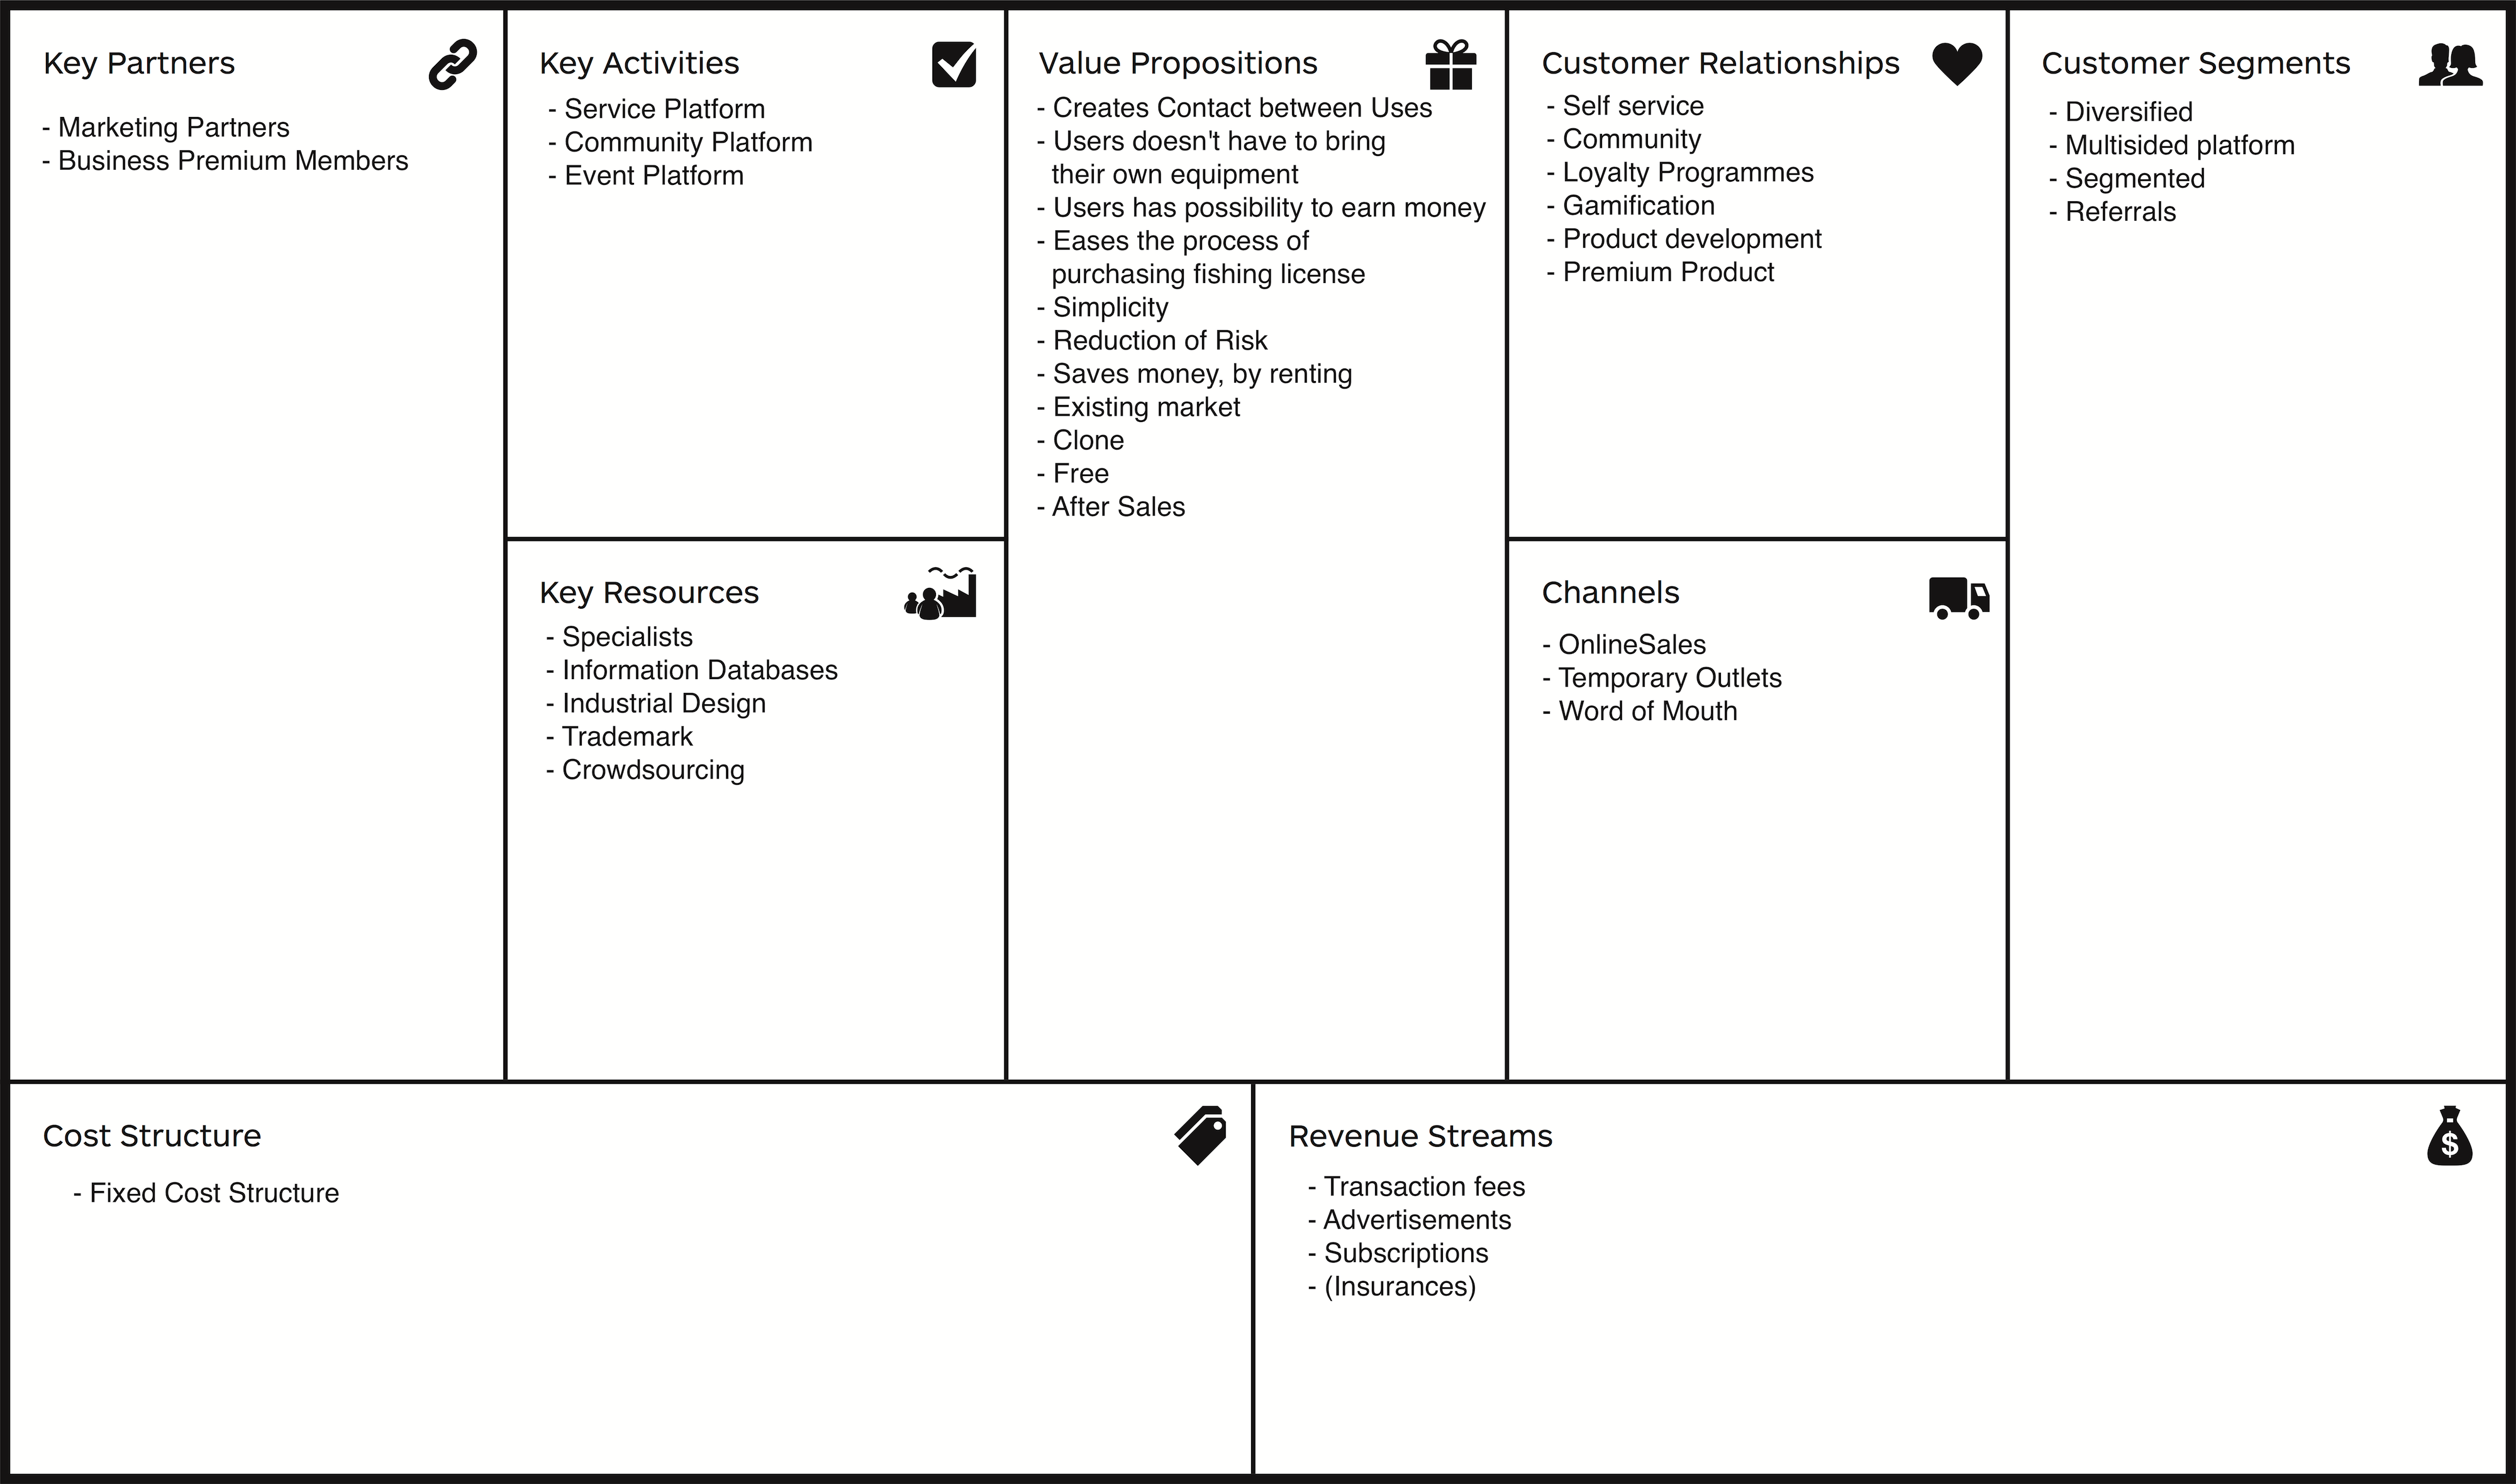
\includegraphics[width=.45\textwidth]{images/business_canvas.png}
  \caption{The Osterwalder Business Canvas}
  \label{fig:bcanvas}
  \footnotesize{\textit{A larger version can be found in appendix \ref{app:bcanvas}}}
\end{figure}

\subsubsection{Customer Segments}
The customers are diversified, as they are served with different products. The users of the platform are served with a free access to the platform, but the businesses on the platform are served, if subscribed, with a advertisement suite, which can be used to approach the users on the platform.

The platform is segmented, and can potentially be expanded into other segments, where it would have other features to suit other outdoor activities and needs.

\subsubsection{Value Proposition Canvas}
The value proposition canvas (shown in \autoref{fig:vpcanvas}) can be used to analyse, what values the product brings to the users. It is based on two elements of the business model: Customer segments and value propositions \cite{vpcanvas}. 

It maps the customers (users) with the product, and shows if there is a fit between them.
\begin{figure}[H]
  \centering
  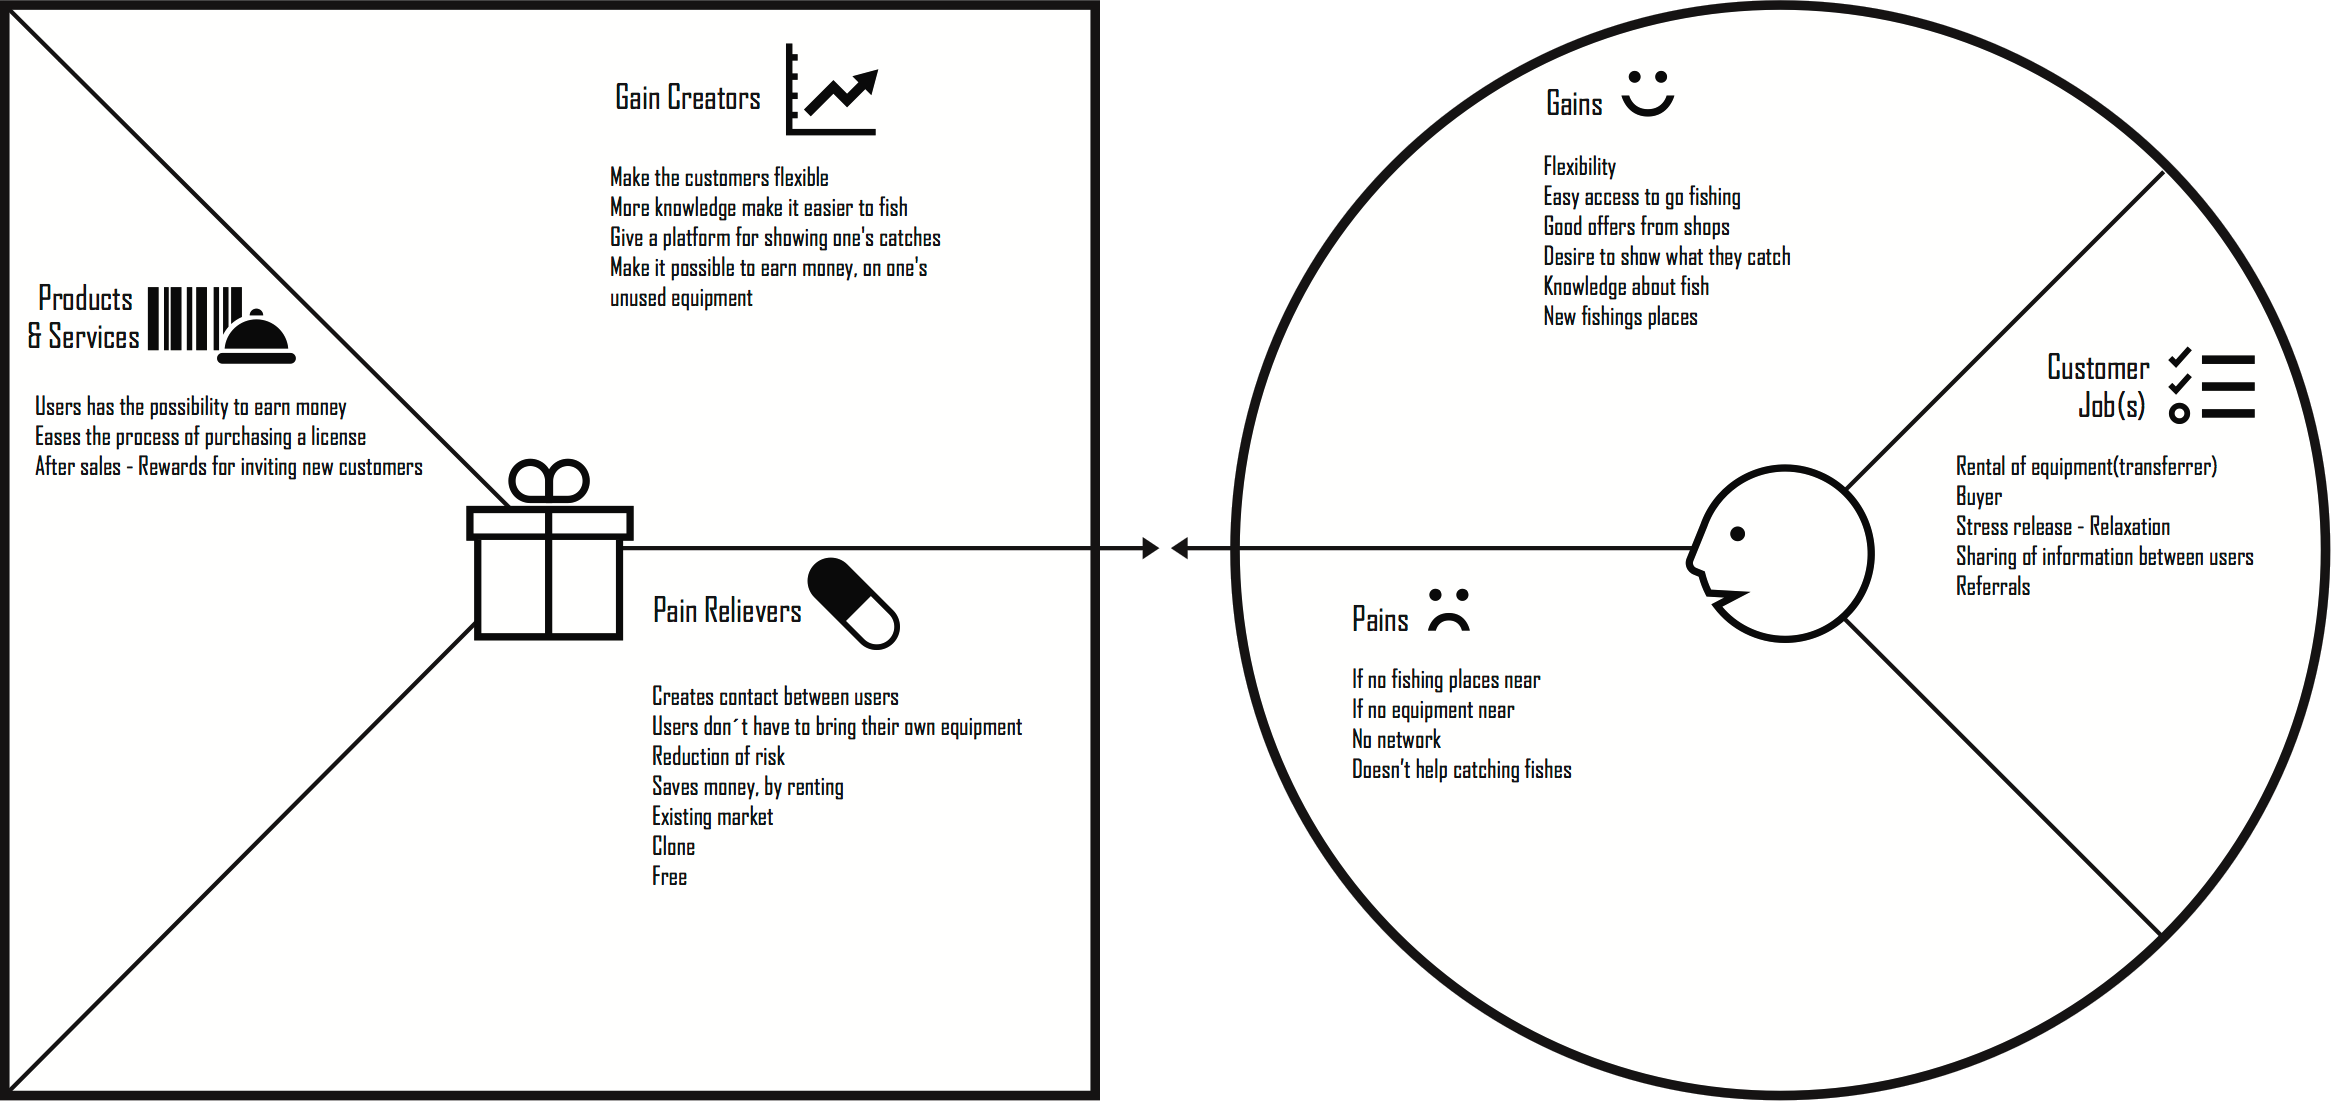
\includegraphics[width=.45\textwidth]{images/value_proposition_canvas.png}
  \caption{The Osterwalder Value Proposition Canvas}
  \label{fig:vpcanvas}
  \footnotesize{\textit{A larger version can be found in appendix \ref{app:vpcanvas}}}
\end{figure}

{\noindent \textbf{Customer Gains\\}}
Customer gains describes the desire, social gain and positive emotions. Some gains are more relevant than others. Tease gains are the ones that are possible to observe in the marked.\\
  
{\noindent \textbf{Customer Pains\\}}
Customer pains describes anything which annoys before, during or after a job is done. This could be undesired cost, negative emotions or risks. Again, some may be more relevant than others. \\

{\noindent \textbf{Customer Jobs\\}}
Customer jobs are the jobs, that the customers are trying to get done, in their job or life. It could be a task or a problem they are trying to solve, or a need they are trying to satisfy. The jobs can have a functional, social or emotional intent. \\

{\noindent \textbf{Gain Creators\\}}
Gain creators tells explicitly, how the product and services creates gains for the customer.\\

{\noindent \textbf{Pain Relievers\\}}
Pain relievers tells explicitly, how the product solves the pains of the customers, before, while or after they are trying to get a job done. It shows which of the customer's pains that the product is solving. \\

{\noindent \textbf{Products and Services\\}}
A simple overview of the products and services, which is provided to the customers, to get a functional, social or emotional job done, and to address their pains and gains. 

\subsubsection{Channel}
The platform will mostly reach the customers via. online sales, as it is a digital platform. Businesses on the platform will also be urged, to refer their current customers to the platform, so that more users will join the platform.\\

The team will strive to be present at outdoor fairs, to gather feedback from current users, but also recruit more users.

\subsubsection{Customer Relationships}
The platform will gain customer relationships, through a variety of attributes. First of all the user is rewarded, for inviting other users to the platform. The customers are able to interact on the platform e.g. by sharing daily catches etc. Through gamification, the platform strengthens the relationship with the customer e.g. with a leaderboard for the largest caught fish. By evaluating reviews and constructive criticism, the platform desires to enhance the product, this will strengthen the customer relationship. A premium version of the product will be available for businesses, which gives them several advantages. This could e.g. be a tag, which indicates that the premium user is verified. A premium users post, will be prioritized in favor of non-premium users.

\subsubsection{Revenue Streams}
The revenue streams of the platform, are the areas which will generate money.\\

The team will take a cut, off of all transactions made on the platform, a flat percentage of 5-10\%.\\

It is possible to allow advertisements, such as google adsense \cite{adsense} on the user app, and the website, to gain an extra amount of money. There could also be a possibility for the user to pay, to not have advertisement on their app, other than the businesses already on the platform.\\

The business premium subscriptions, will also bring in a vast majority of the money earned on the platform.\\

It could also be lucrative to sell an insurance, for the rented equipment, so that the owner will get the cost of his equipment covered, in case it breaks or gets lost, during a rental.

\subsubsection{Key Activities}
The key activities of the team, is to provide the platform.

The team provides a platform where: 
\begin{itemize}
	\item Other businesses can connect to their customers, and create events and promote their sales.
	\item Individual users can connect with like-minded users, to share ideas, tips, equipment and experiences.
	\item Users have the ability to start events, such as a fishing tournament, to meet each other.
\end{itemize}

\subsubsection{Key Resources}
The Key resources to make the app function, are:
\begin{itemize}
	\item Specialists - The business needs specialists, to get off ground and create the application.
	\item Information databases - The business depends on having information about the users, their behaviors, and how they navigate and respond on the application.
	\item Industrial design - The user interface of the application needs to be as convenient as possible, to make it feel natural for the user to use.
	\item Trademark - It is vital that our brand is not misrepresented/ruined.
	\item Crowdsourcing - The vast majority of the content on the platform is going to be crowdsourced, by the users (events and rentals/businesses).
\end{itemize}

\subsubsection{Key Partners}
The key partners will be other businesses, as marketing partners, they will refer their customers to the platform, and the platform will in exchange make the users aware of the businesses.

\subsubsection{Cost Structure}
The cost of implementing and maintaining the business, has a fixed costs.The business has relatively fixed costs (wages), and can't adapt our expenses to the minimum income of the product. When the business grows, the cost will grow as well. The biggest cost growth, is the wages for the staff, which grows 30.000 DKK. every year. 
